% !TeX encoding = UTF-8
\documentclass[12pt, a4paper]{article}

\usepackage{geometry}
\usepackage{amsmath, amsfonts, amssymb, amsthm} % стандартный набор AMS-пакетов для математ. текстов
\usepackage{mathtext}
\usepackage[utf8]{inputenc} % кодировка utf8
\usepackage[russian]{babel} % русский язык
\usepackage[pdftex,dvipsnames]{xcolor} % работа с цветами
\usepackage[pdftex]{graphicx} % графика (картинки)
\usepackage{tikz,pgfplots} % рисунки
\usepackage{booktabs}
\usepackage{indentfirst}
%\usepackage[labelfont=bf,labelsep=endash,skip=3pt]{caption} % подпись картинок
% \usepackage{fancyhdr,pageslts} % настройка колонтитулов
\usepackage{enumitem} % работа со списками
\usepackage{floatrow,multicol,multirow,longtable,hhline} % работа с таблицами
\usepackage{float,wrapfig} % плавающие объекты
\usepackage{tcolorbox} % рамка вокруг текста
%\usepackage[calc]{datetime2} % дата
\usepackage{bm} % жирное начертание в формулах
\usepackage{physics} % физический пакет
\DeclareMathAlphabet\mathbfcal{OMS}{cmsy}{b}{n}
\usepackage{pgfornament} % красивые рюшечки и вензеля
\usepackage{mdframed}
\usepackage{derivative}
\usepackage{mathrsfs} %EDS
\usepackage{soul} % strikethorugh

%\usepackage{boondox-cal}

% ----------------------------------------
% Настройка шрифта

% Просто закооментируйте следующую строчку, если не работает. Будет другой шрифт, правда :(
% \usepackage{pscyr}

% ----------------------------------------
% Стилевые настройки

\usepackage{boldline} % жирная линия после таблиц (чтобы не было ошибок, этот пакет должен подключаться именно тут!)
\floatsetup[table]{style=Plaintop,floatrowsep=qquad} % настройка оформления таблиц
\setlist[enumerate,itemize]{leftmargin=5mm,itemindent=10mm,itemsep=0mm,
listparindent=0em,labelsep=2mm,topsep=2mm,labelwidth=4mm} % настройки списков

\setlength{\columnsep}{0.5cm} % расстояние между колонками
\setlength{\parskip}{1pt} % расстояние до текста от колонтитула

%\usepackage{titlesec} % управление оформлением section
%\renewcommand{\thesection}{\Roman{section}}
%\titleformat{\section}[block]{\bfseries\large}{\thesection.}{5pt}{}

% Настройка совместимости
\pgfplotsset{compat=1.18}

% ----------------------------------------
% Настройки полей
\geometry{
	left=10mm,
	top=10mm,
	right=10mm,
	bottom=15mm,
	marginparsep=0mm,
	marginparwidth=0mm,
	headheight=0pt,
	headsep=0pt,
	footskip=20pt}

% ----------------------------------------
% Настройки колонтитулов и нумерации страниц
\pagenumbering{arabic}



\newcounter{ntask}
\setcounter{ntask}{0}


\newcommand{\arsh}{\mathrm{arsh} \,\,}
\newcommand{\arch}{\mathrm{arch} \,\,}
\newcommand{\arth}{\mathrm{arth} \,\,}
\newcommand{\arcth}{\mathrm{arcth} \,\,}
\renewcommand{\Re}{\operatorname{Re} \,}
\newcommand{\EDS}{\mathscr{E}}
\newcommand{\diffract}[1]{\frac{\mathrm{d}#1}{\mathrm{d}t}}

\newcommand{\kHz}{~\mathrm{kHz}}
\newcommand{\GHz}{~\mathrm{GHZ}}
\newcommand{\us}{~\mathrm{\mu s}}
\addto\captionsrussian{\def\refname{Источники}}

\begin{document}
\title{\begin{center}Лабораторная работа № 5.4.1\end{center}
Определение энергии $\alpha$-частиц по велечине их пробега в воздухе}
\author{Струков О. И. \\ Б04-404}
\date{}

\thispagestyle{empty}
\pagenumbering{gobble}
\maketitle
\newpage
\pagenumbering{arabic}



\section*{Теоретическая часть}

\subsection*{1. Альфа-распад и правило Гейгера-Неттола}
При $\alpha$-распаде исходное родительское ядро испускает ядро гелия ($\alpha$-частицу) и превращается в дочернее ядро, число протонов и число нейтронов которого уменьшается на две единицы. Периоды полураспада $\alpha$-активных ядер изменяются в чрезвычайно широких пределах (от долей секунды до миллиардов лет), тогда как диапазон энергии вылетающих $\alpha$-частиц значительно меньше и составляет от 4 до 9 МэВ. При этом наблюдается закономерность: чем меньше энергия $\alpha$-частиц, тем больше период полураспада. 

Функциональная связь между энергией $\alpha$-частицы $E$ и периодом полураспада $T_{1/2}$ хорошо описывается эмпирической формулой Гейгера-Неттола:
\begin{equation}
    \lg T_{1/2} = \frac{a}{\sqrt{E}} + b,
\end{equation}
Теоретическое обоснование этого закона было получено после создания квантовой механики. Они показали, что вероятность вылета $\alpha$-частицы из ядра определяется вероятностью её проникновения сквозь кулоновский барьер (туннельный эффект). Экспоненциальный характер этого процесса возникает вследствие экспоненциального затухания волновой функции в области под барьером.

\subsection*{2. Взаимодействие тяжёлых заряженных частиц с веществом}
Тяжелые заряженные частицы (протоны, $\alpha$-частицы) при прохождении через вещество теряют свою энергию главным образом в результате неупругих столкновений с атомами среды, вызывая их ионизацию и возбуждение. Поскольку в каждом акте столкновения передается малая доля энергии (не более $4mE/M$), траектория частицы остается практически прямолинейной.

Расчёт удельных потерь энергии на ионизацию в классическом приближении был проведен Н. Бором. Для нерелятивистской тяжелой частицы с зарядом $z$ и скоростью $v$ формула имеет вид:
\begin{equation}
    \left(\frac{dE}{dx}\right)_{ион} \simeq \frac{2\pi e^4 z^2}{m v^2} n Z \ln\left(\frac{2mv^2}{I}\right),
\end{equation}
где $m$ --- масса электрона, $n$ --- плотность атомов среды, $Z$ --- заряд атома среды, $I$ --- средний ионизационный потенциал. Величина $dE/dx$ называется тормозной способностью вещества. Из формулы видно, что при данном заряде потери энергии определяются только скоростью частицы: быстрее всего теряют энергию медленные частицы.

Зависимость $dE/dx$ от пути, пройденного частицей в веществе, носит название \textbf{кривой Брэгга}. В конце пробега кривая имеет характерный подъём, называемый пиком Брэгга.

% === МЕСТО ДЛЯ ВСТАВКИ ГРАФИКА ===
\begin{figure}[htbp]
    \centering
    
\includegraphics[width=0.5\textwidth]{1.jpg} % Раскомментируйте и укажите имя файла
    % \fbox{\parbox{0.7\textwidth}{\centering\vspace{2cm} \textit{Вставьте сюда Рис. 1 из методички: Кривые Брэгга для $\alpha$-частиц} \vspace{2cm}}}
    \caption{Кривые Брэгга для $\alpha$-частиц, испускаемых $^{210}$Po и $^{214}$Po.}
    \label{fig:bragg}
\end{figure}

\subsection*{3. Пробег альфа-частиц}
Путь тяжёлых заряженных частиц в веществе практически прямолинеен, а разброс длин путей невелик, поэтому можно говорить о длине пробега $R$. Зная тормозную способность, можно вычислить длину пробега частицы. Однако теоретические формулы недостаточно точно описывают экспериментальные данные, поэтому для связи энергии $\alpha$-частицы и её пробега в воздухе используют эмпирическое соотношение (в диапазоне энергий от 4 до 9 МэВ):
\begin{equation}
    R = 0,32 E^{3/2},
\end{equation}
где пробег $R$ выражается в сантиметрах (при $15^\circ$C и нормальном атмосферном давлении), а энергия $E$ --- в МэВ.

Энергию частиц удобнее определять не геометрическим пробегом в сантиметрах, а массовым пробегом $R' = \rho R$, имеющим размерность г/см$^2$. 

Из-за рассеяния и статистического характера потерь энергии пробеги разных $\alpha$-частиц с одинаковой начальной энергией несколько отличаются. На практике используют \textbf{средний пробег} $R_{ср}$ и \textbf{экстраполированный пробег} $R_э$, который находится путем продолжения касательной к кривой $N(x)$ в точке $x = R_{ср}$ до пересечения с осью абсцисс.

% === МЕСТО ДЛЯ ВСТАВКИ ГРАФИКА ===
\begin{figure}[htbp]
    \centering
    
\includegraphics[width=0.5\textwidth]{2.jpg} % Раскомментируйте и укажите имя файла
    % \fbox{\parbox{0.7\textwidth}{\centering\vspace{2cm} \textit{Вставьте сюда Рис. 2 из методички: Зависимость числа $\alpha$-частиц от глубины проникновения} \vspace{2cm}}}
    \caption{Зависимость числа $\alpha$-частиц от глубины их проникновения в вещество.}
    \label{fig:range}
\end{figure}

\subsection*{4. Экспериментальные методы измерения пробега}
В данной работе пробег $\alpha$-частиц определяется тремя различными методами:

\textbf{I. Метод с использованием торцевого счётчика Гейгера.}
Радиоактивный источник помещается на дно стальной бомбы, внутри которой может перемещаться торцевой счетчик Гейгера. Его чувствительный объем отделён от внешней среды тонким слюдяным окошком. Изменяя расстояние между источником и счётчиком, снимают зависимость скорости счёта $N$ от расстояния $x$.

% === МЕСТО ДЛЯ ВСТАВКИ СХЕМЫ ===
\begin{figure}[htbp]
    \centering
    
\includegraphics[width=0.3\textwidth]{3.jpg}
    % \fbox{\parbox{0.6\textwidth}{\centering\vspace{2cm} \textit{Вставьте сюда Рис. 3: Установка для измерения пробега с помощью счетчика Гейгера} \vspace{2cm}}}
    \caption{Схема установки с торцевым счётчиком Гейгера.}
    \label{fig:geiger}
\end{figure}

\textbf{II. Метод с использованием сцинтилляционного счётчика.}
Установка представляет собой цилиндрическую камеру с люминофором на стеклянной пластинке и фотоэлектронным умножителем (ФЭУ). Расстояние между препаратом и люминофором фиксировано (9 см), поэтому $\alpha$-частицы не могут достичь его при обычном давлении. Пробег определяется путём измерения зависимости интенсивности счёта $N$ от давления $P$ воздуха в камере (при откачке или напуске воздуха).

% === МЕСТО ДЛЯ ВСТАВКИ СХЕМЫ ===
\begin{figure}[htbp]
    \centering
    
\includegraphics[width=0.3\textwidth]{4.jpg}
    % \fbox{\parbox{0.6\textwidth}{\centering\vspace{2cm} \textit{Вставьте сюда Рис. 4: Установка со сцинтилляционным счетчиком} \vspace{2cm}}}
    \caption{Схема установки со сцинтилляционным счётчиком.}
    \label{fig:scint}
\end{figure}

\textbf{III. Метод с использованием ионизационной камеры.}
Ионизационная камера представляет собой наполненный газом сосуд с двумя электродами. При прохождении $\alpha$-частиц в газе образуются ионы, которые создают измеримый ток. Камера работает в токовом режиме на «плато» вольтамперной характеристики, где рекомбинация ионов пренебрежимо мала. Измеряя ионизационный ток $I$ в зависимости от давления $P$ в сферической камере, находят экстраполированный пробег $\alpha$-частиц.

% === МЕСТО ДЛЯ ВСТАВКИ СХЕМ И ГРАФИКОВ ===
\begin{figure}[htbp]
    \centering
    
\includegraphics[width=0.4\textwidth]{5.jpg}
    % \fbox{\parbox{0.8\textwidth}{\centering\vspace{2cm} \textit{Вставьте сюда Рис. 5 и Рис. 6 из методички: Схема ионизационной камеры и ее вольтамперная характеристика / зависимость тока от давления} \vspace{2cm}}}
    \caption{Схема ионизационной камеры и характерная кривая зависимости тока от давления.}
    \label{fig:ion}
\end{figure}

\subsection*{5. Бета-распад}
Помимо альфа-распада, в ядерной физике исследуется бета-распад --- самопроизвольное превращение ядер, при котором их массовое число не изменяется, а заряд увеличивается или уменьшается на единицу. В случае электронного $\beta^-$-распада происходит превращение:
\begin{equation}
    ^A_Z X \rightarrow ^A_{Z+1} X + e^- + \tilde{\nu},
\end{equation}
где наряду с электроном испускается электронное антинейтрино $\tilde{\nu}$. Освобождающаяся энергия делится между электроном, антинейтрино и дочерним ядром. Поскольку доля энергии, передаваемой ядру, ничтожно мала, электрон и антинейтрино делят энергию между собой. В результате электроны могут иметь любое значение энергии --- от нулевой до некоторой максимальной ($E_{max}$), которая равна полной энергии, освобождающейся при $\beta$-распаде, и является важной физической величиной, определяемой в лабораторном практикуме с помощью магнитного спектрометра.

















\section*{Ход работы}

\subsection*{Часть 1. Исследование пробега $\alpha$-частиц с помощью торцевого счётчика Гейгера}

В ходе эксперимента измерялась зависимость скорости счёта $\alpha$-частиц $n$ от расстояния $x$ между источником ($^{239}$Pu) и торцевым счётчиком Гейгера.% Время измерения в каждой точке составляло $t = \dots$ с. Фоновый счет составил $n_{bg} = \dots$ имп/с.

Результаты измерений представлены в таблице 1:% Статистическая погрешность рассчитывалась по формуле $\Delta n = \sqrt{n/t}$.

\begin{table}[H]
\centering

\renewcommand{\arraystretch}{1.3} % Немного увеличим высоту строк для читаемости
\begin{tabular}{|c|c|c|c|}
\hline
$x$, мм & $N_{\text{ср}}$, имп/с & $\sigma_N$, имп/с & $\sigma_x$, мм \\
\hline
0    & 16,200 & 1,273 & 0,5 \\
2,5  & 18,750 & 1,369 & 0,5 \\
5    & 14,850 & 1,219 & 0,5 \\
6    & 13,833 & 1,176 & 0,5 \\
7,5  & 4,500  & 0,671 & 0,5 \\
9    & 0,433  & 0,208 & 0,5 \\
10   & 0,483  & 0,220 & 0,5 \\
12,5 & 0,233  & 0,153 & 0,5 \\
15   & 0,467  & 0,216 & 0,5 \\
20   & 0,121  & 0,110 & 0,5 \\
25   & 0,250  & 0,158 & 0,5 \\
30   & 0,098  & 0,099 & 0,5 \\
35   & 0,150  & 0,122 & 0,5 \\
40   & 0,100  & 0,100 & 0,5 \\
\hline
\end{tabular}
\caption{Зависимость скорости счёта $\alpha$-частиц от расстояния до источника}
\label{tab:geiger_data}
\vspace{0.2cm}
% \begin{minipage}{0.9\textwidth}
% \footnotesize
% \end{minipage}
\end{table}

По полученным данным был построен график зависимости $N(x)$ с учётом погрешностей:
\begin{figure}[H]
    \centering
    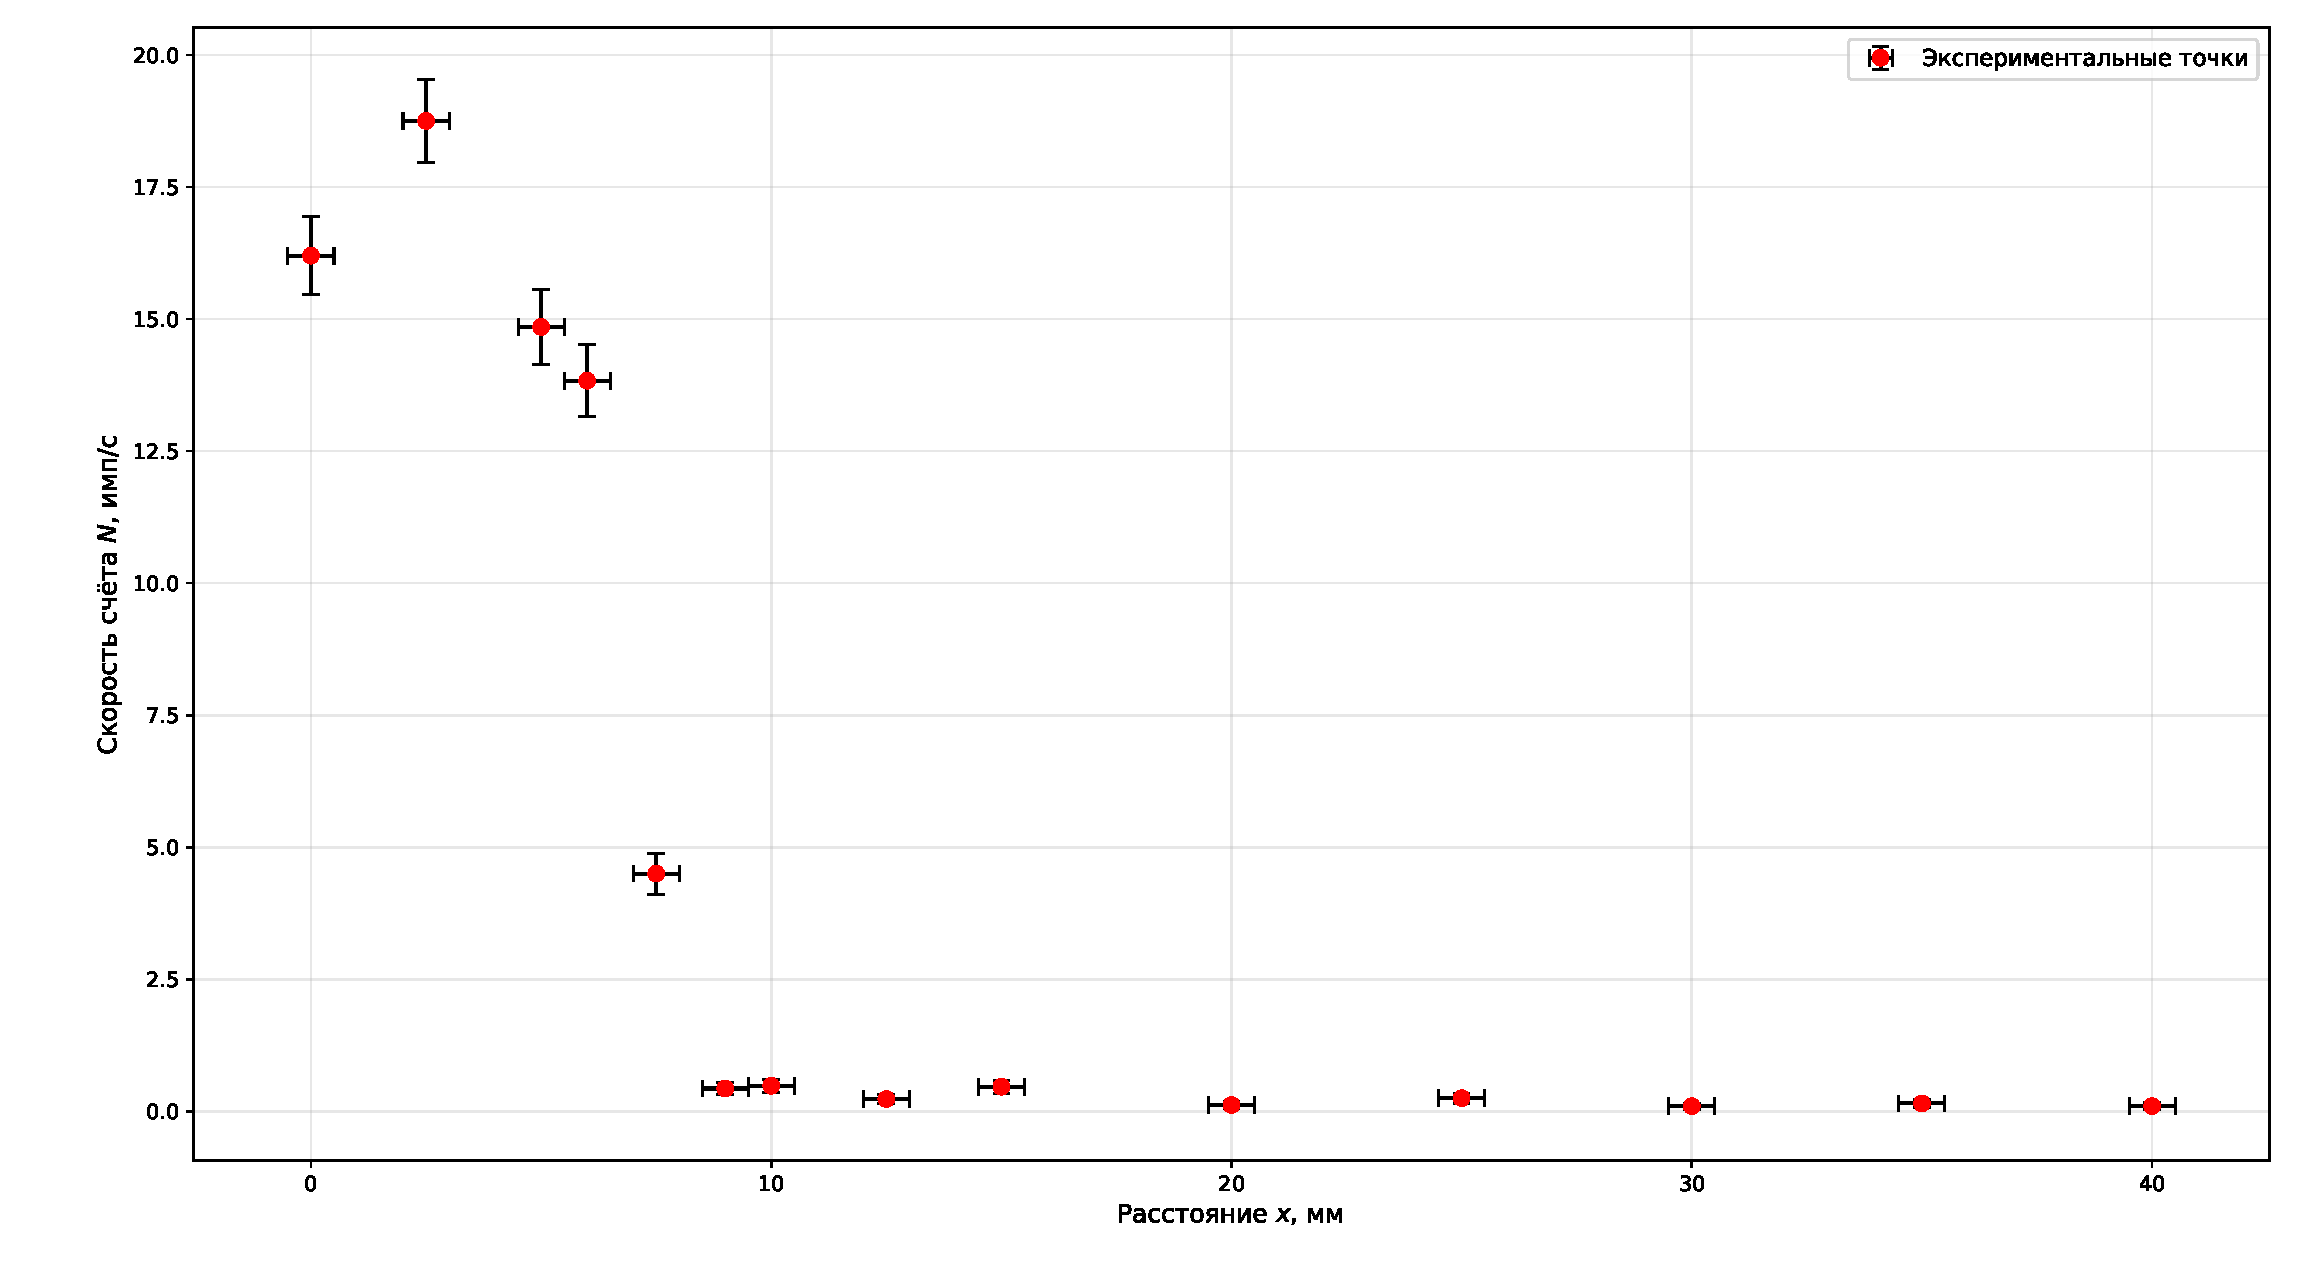
\includegraphics[width=0.8\textwidth]{7.pdf}
    % \fbox{\parbox{0.8\textwidth}{\centering\vspace{3cm} \textit{Вставьте сюда график N(x) с ошибочными полосами (error bars). \\ На графике должны быть отмечены уровни плато, спада и фона.} \vspace{3cm}}}
    \caption{Зависимость скорости счёта $\alpha$-частиц от расстояния до источника в линейном масштабе.}
\end{figure}

% === МЕСТО ДЛЯ ГРАФИКА N(x) ===
\begin{figure}[H]
    \centering
    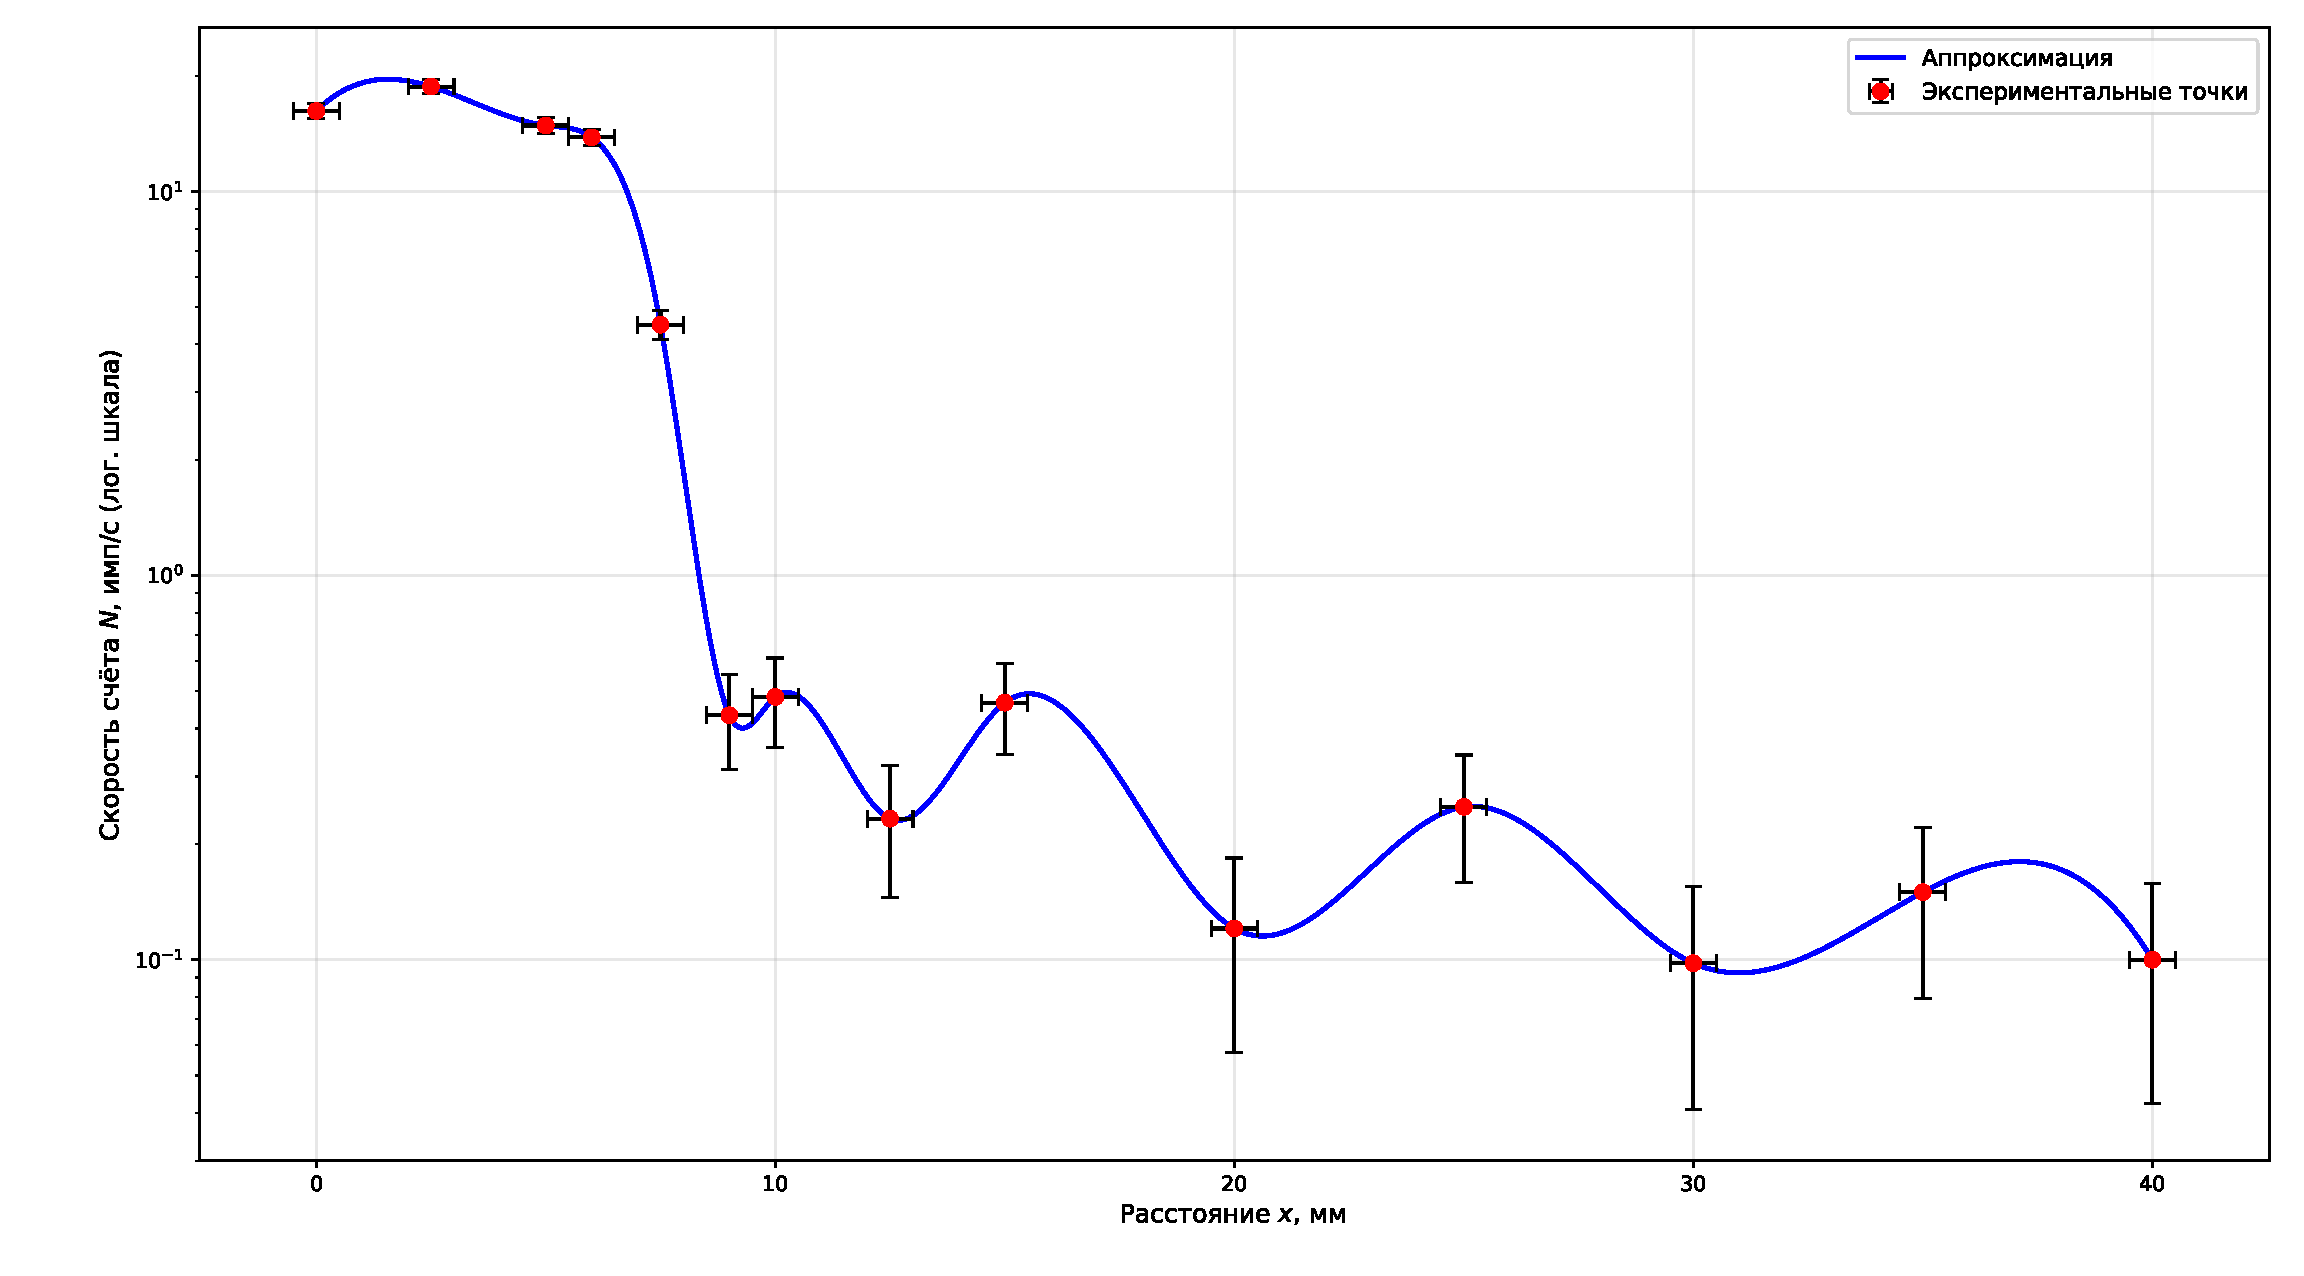
\includegraphics[width=0.8\textwidth]{6.pdf}
    % \fbox{\parbox{0.8\textwidth}{\centering\vspace{3cm} \textit{Вставьте сюда график N(x) с ошибочными полосами (error bars). \\ На графике должны быть отмечены уровни плато, спада и фона.} \vspace{3cm}}}
    \caption{Зависимость скорости счёта $\alpha$-частиц от расстояния до источника с логарифмической шкалой.}
    \label{fig:geiger_graph}
\end{figure}



По графику были определены значения среднего и экстраполированного пробега $\alpha$-частиц в воздухе:
\begin{itemize}
    \item Средний пробег: $R_{ср} \approx 0,75$ см.
    \item Экстраполированный пробег: $R_{э} \approx 0,81$ см.
\end{itemize}

Для перехода к массовому пробегу $R'$ (г/см$^2$) использовались плотность воздуха при $T = 15^\circ$C и нормальном давлении $\rho \approx 1,226 \cdot 10^{-3}$ г/см$^3$:
\begin{equation}
    R' = \rho R.
\end{equation}
Тогда массовый пробег составляет:
\begin{equation}
    R'_{ср} \approx 9,20 \cdot 10^{-4} \text{ г/см}^2, \quad R'_{э} \approx 9,93 \cdot 10^{-4} \text{ г/см}^2.
\end{equation}
% \textit{Примечание:} Истинный пробег $\alpha$-частиц в воздухе больше измеренного, так как часть энергии теряется при прохождении защитной пленки источника и слюдяного окошка счетчика. 

% Энергию $\alpha$-частиц $E$ (в МэВ) вычислим по эмпирической формуле $R = 0,32 E^{3/2}$, выразив $E$ через $R$ (в см):
% \begin{equation}
%     E = \left( \frac{R}{0.32} \right)^{2/3}.
% \end{equation}

% Подставляя найденные значения пробега, получаем:
% \begin{equation}
%     E_{ср} = \dots \text{ МэВ}, \quad E_{э} = \dots \text{ МэВ}.
% \end{equation}

% Погрешность определения энергии рассчитаем через производную:
% \begin{equation}
%     \Delta E = \left| \frac{dE}{dR} \right| \Delta R = \frac{2}{3} \frac{E}{R} \Delta R.
% \end{equation}
% \begin{equation}
%     \Delta E_{ср} = \dots \text{ МэВ}, \quad \Delta E_{э} = \dots \text{ МэВ}.
% \end{equation}

% Итоговый результат для энергии $\alpha$-частиц $^{239}$Pu:
% \begin{equation}
%     E = \dots \pm \dots \text{ МэВ}.
% \end{equation}
% Табличное значение энергии для $^{239}$Pu составляет $E_{табл} = 5,15$ МэВ. Расхождение составляет $\dots$ \%, что находится в пределах погрешности / указывает на необходимость учета поправки на поглощение в слюде.




\subsection*{Часть 2. Исследование пробега $\alpha$-частиц с помощью сцинтилляционного счётчика}

Расстояние между источником $^{239}\text{Pu}$ и люминофором составляло $L = 9$ см. Рабочее напряжение на фотоэлектронном умножителе $U = 1100$ В. Атмосферное давление $P_{\text{атм}} = 743,2$ мм рт. ст., температура в лаборатории $T_{\text{}} \approx 293$ К. 

Определение пробега сводится к измерению зависимости скорости счёта $N$ от абсолютного давления воздуха $P$ в камере. При снижении давления плотность воздуха уменьшается, и $\alpha$-частицы получают возможность достигать детектора. Результаты измерений представлены в таблице 2:

\begin{table}[H]
\centering

\renewcommand{\arraystretch}{1.2}
\begin{tabular}{|c|c|c|c|c|}
\hline
$P$, мм рт. ст. & $N_{\text{част}}$ (за 10 с) & $N$, имп/с & $\sigma_N$, имп/с & $\sigma_ P$, мм рт. ст. \\
\hline
21   & 3244 & 324,4 & 5,70 & 1 \\
58   & 2548 & 254,8 & 5,05 & 1 \\
93   & 1896 & 189,6 & 4,35 & 1 \\
121  & 1356 & 135,6 & 3,68 & 1 \\
143  &  959 &  95,9 & 3,10 & 1 \\
195  &  326 &  32,6 & 1,81 & 1 \\
243  &   92 &   9,2 & 0,96 & 1 \\
293  &   31 &   3,1 & 0,56 & 1 \\
343  &    3 &   0,3 & 0,17 & 1 \\
393  &    3 &   0,3 & 0,17 & 1 \\
443  &    4 &   0,4 & 0,20 & 1 \\
543  &    6 &   0,6 & 0,24 & 1 \\
593  &    4 &   0,4 & 0,20 & 1 \\
693  &    2 &   0,2 & 0,14 & 1 \\
743  &    1 &   0,1 & 0,10 & 1 \\
\hline
\end{tabular}
\caption{Зависимость скорости счёта $\alpha$-частиц от давления воздуха}
\label{tab:scint_data}
\end{table}

По полученным данным был построен график зависимости $N(P)$:

\begin{figure}[H]
    \centering
    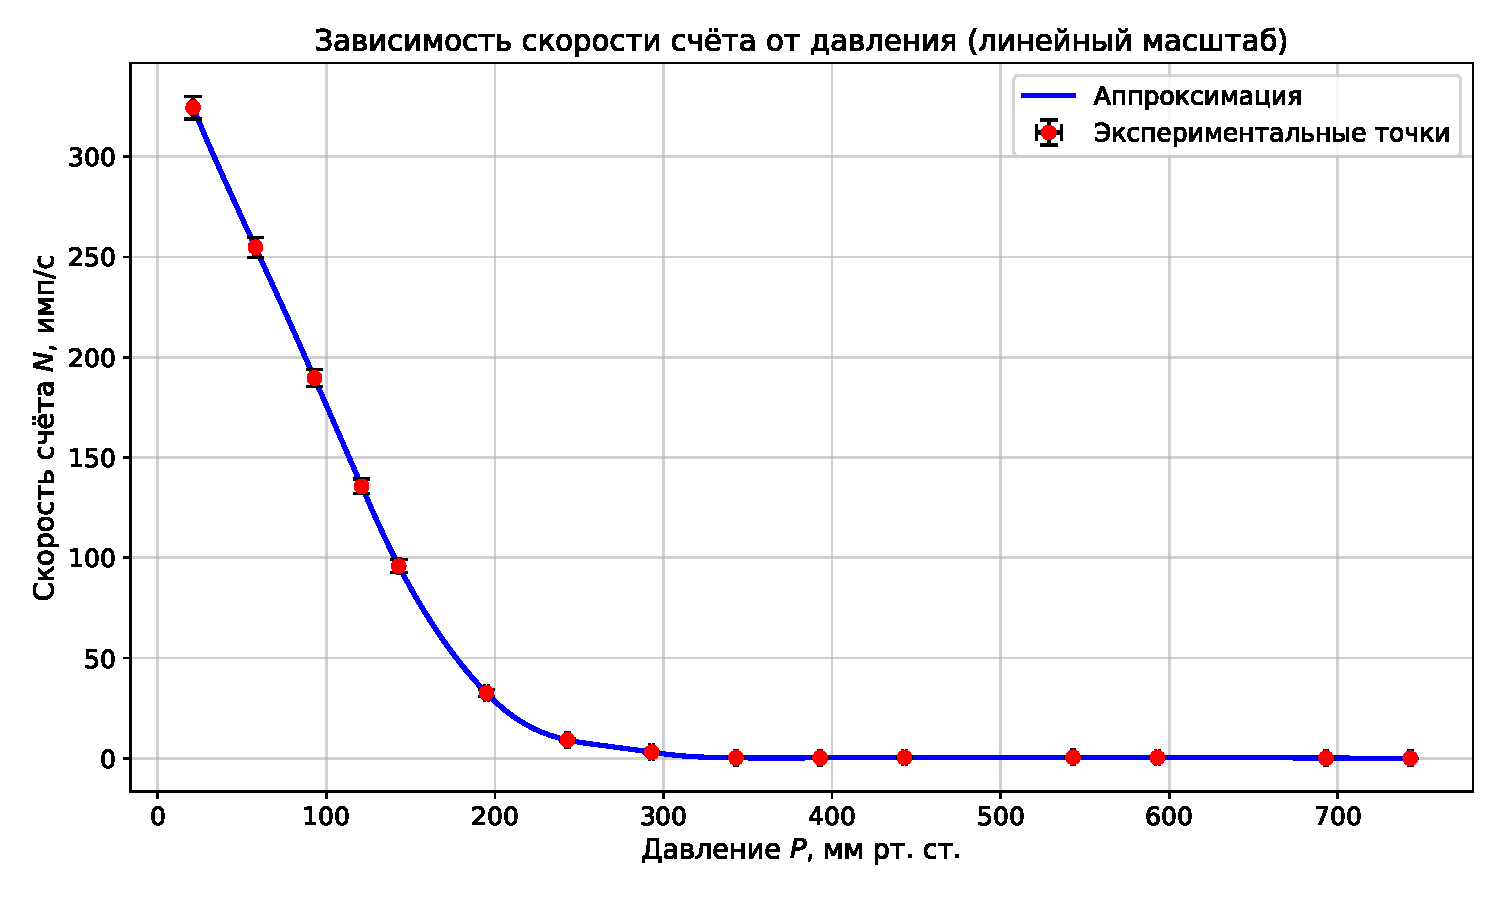
\includegraphics[width=0.8\textwidth]{81.pdf}
    \caption{Зависимость скорости счёта $\alpha$-частиц от давления воздуха.}
    \label{fig:scint_log}
\end{figure}

% \begin{figure}[H]
%     \centering
%     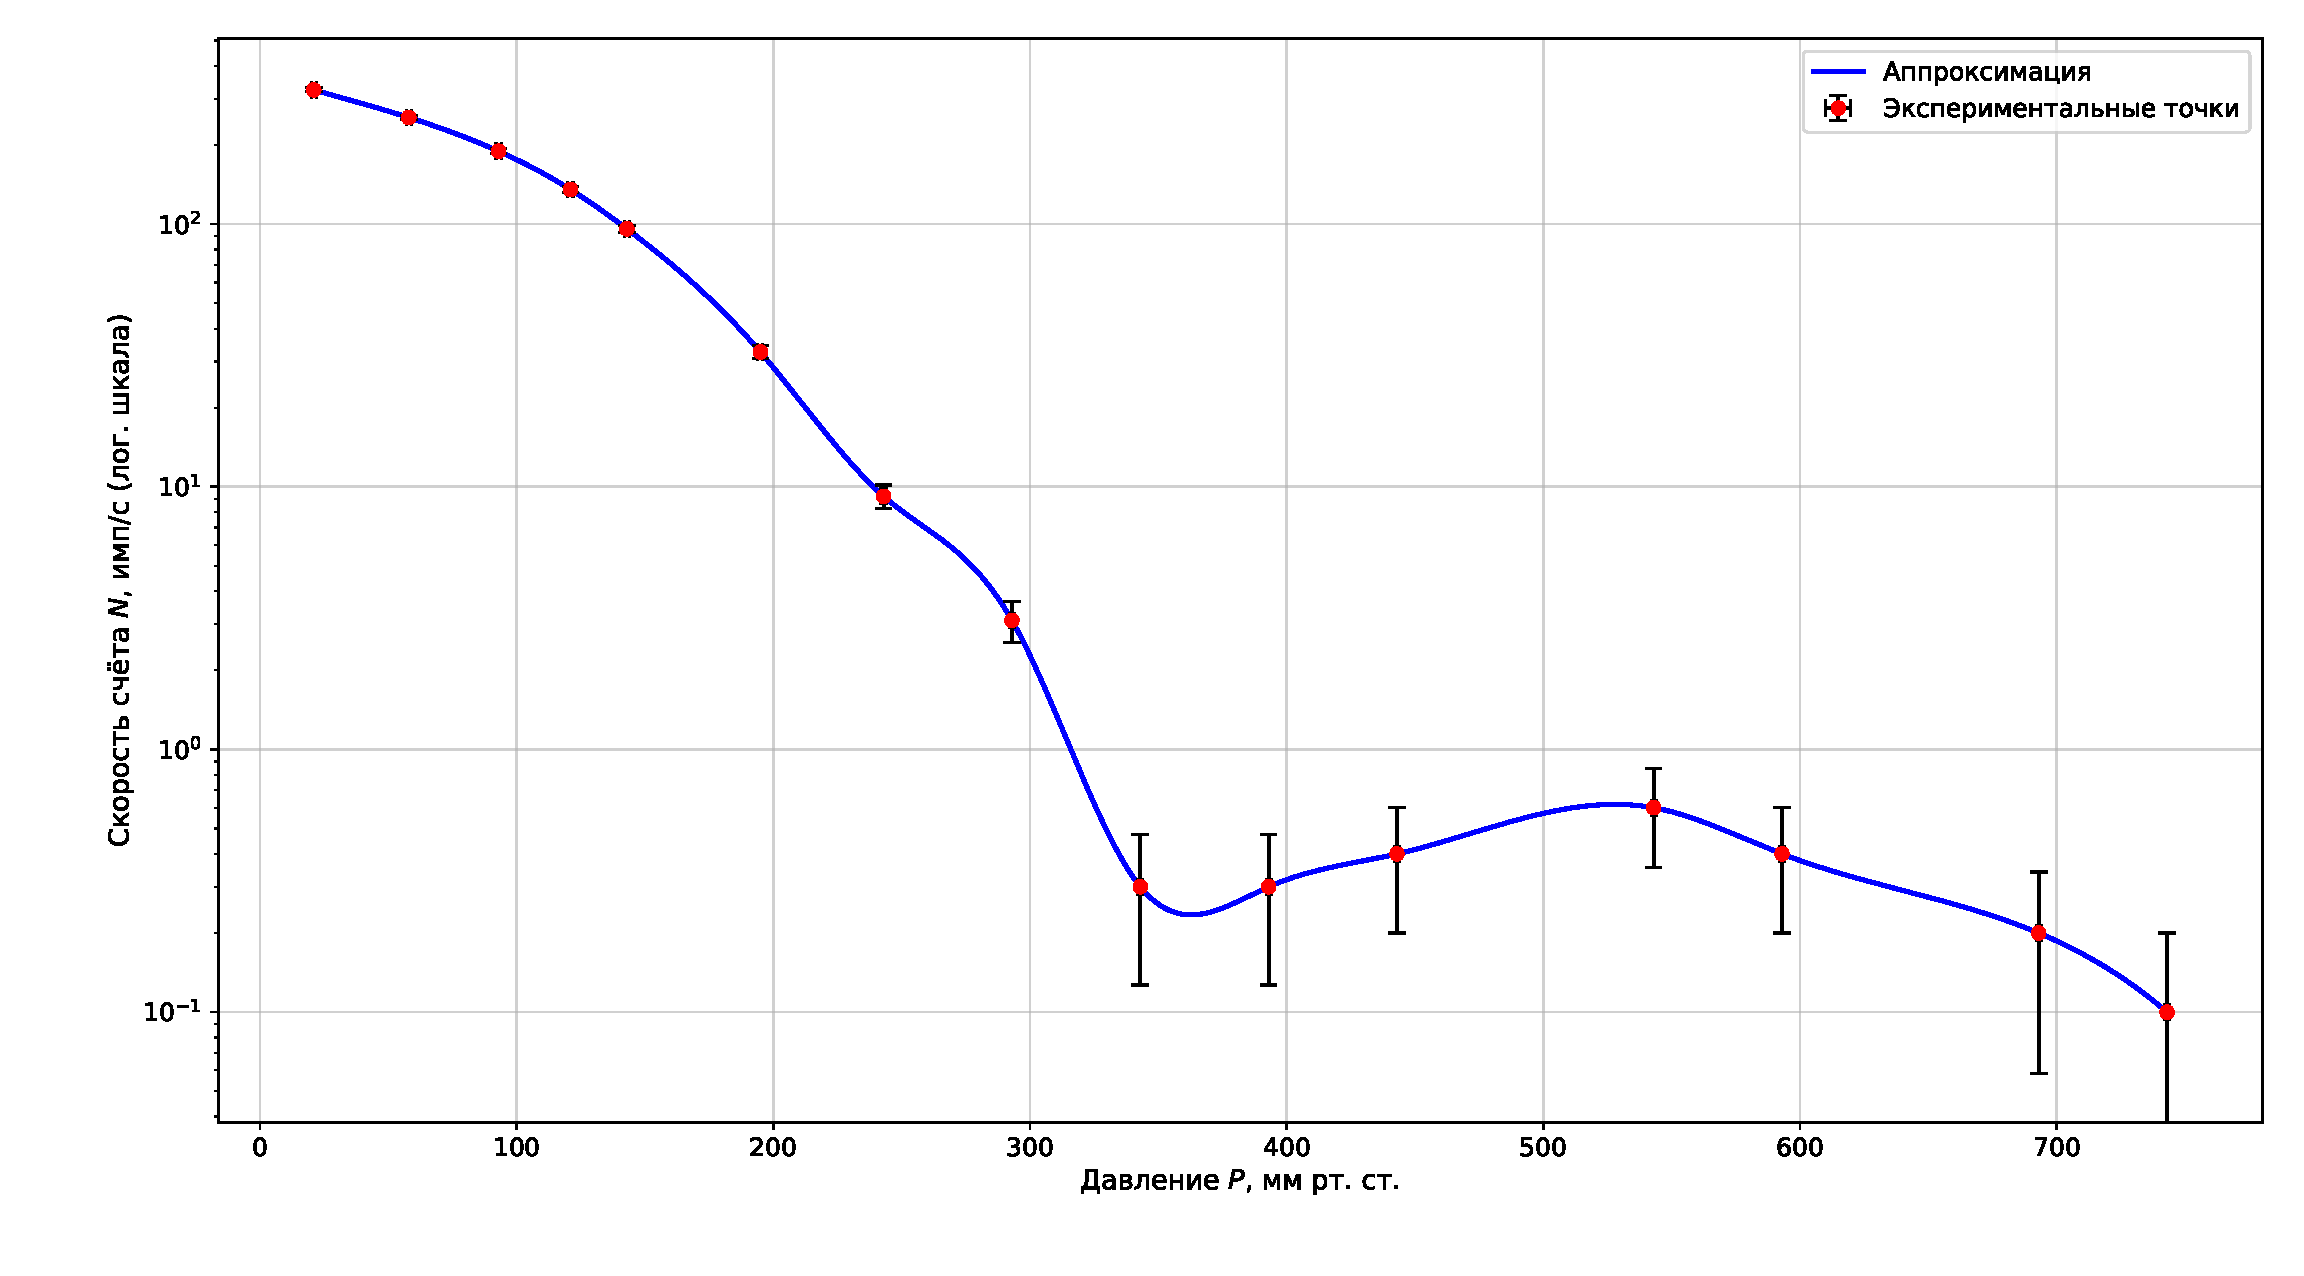
\includegraphics[width=0.8\textwidth]{8.pdf}
%     \caption{Зависимость скорости счёта $\alpha$-частиц от давления воздуха.}
% \end{figure}

% \begin{figure}[H]
%     \centering
%     \includegraphics[width=0.8\textwidth]{scint_linear_drop_smooth.png}
%     \caption{Определение экстраполированного давления $P_{\text{э}}$ по линейному участку спада кривой.}
%     \label{fig:scint_drop}
% \end{figure}

\subsubsection*{Обработка результатов и пересчёт к нормальным условиям}
Из графика на Рис. \ref{fig:scint_log} методом экстраполяции линейного участка спада до уровня фона ($N \approx 0,33$ имп/с) было определено критическое давление $P_{\text{кр}}$, при котором $\alpha$-частицы перестают достигать люминофора:
\begin{equation}
    P_{\text{кр}} \approx 194 \text{ мм рт. ст.}
\end{equation}

Поскольку геометрическая длина пробега в установке равна $L = 9$ см, истинный линейный пробег $R_0$ при нормальных условиях ($P_0 = 760$ мм рт. ст., $T_0 = 15^\circ\text{C} = 288$ К) вычисляется по формуле:
\begin{equation}
    R_0 = L \cdot \frac{P_{\text{кр}}}{P_0} \cdot \frac{T_0}{T_{\text{оп}}} \approx 2,42 \text{ см}.
\end{equation}

Массовый пробег при нормальных условиях ($\rho_0 \approx 1,226 \cdot 10^{-3}$ г/см$^3$):
\begin{equation}
    R'_0 = \rho_0 R_0 \approx 2,97 \cdot 10^{-3} \text{ г/см}^2 = 2,97 \text{ мг/см}^2.
\end{equation}

Полученные значения пробега существенно различаются: $R_{\text{Гейгер}} \approx 0{,}81$ см и $R_{\text{сцинт}} \approx 2{,}42$ см. Основная причина расхождения — поглощение $\alpha$-частиц в слюдяном окошке торцевого счётчика Гейгера, которое отсутствует в сцинтилляционной установке.% Метод сцинтилляционного счетчика точнее, так как исключает эту систематическую погрешность; статистическая погрешность обоих методов определяется законом Пуассона и составляет несколько процентов.


\subsubsection*{Оценка толщины слюдяного окошка }
Сравнивая массовый пробег, полученный на сцинтилляционном счётчике ($R'_{0, \text{сцинт}} = 2,97$ мг/см$^2$), с массовым пробегом из части 1 ($R'_{0, \text{Гейгер}} \approx 0,99$ мг/см$^2$), можно найти потерю пробега на преодоление слюдяного окошка торцевого счётчика Гейгера:
\begin{equation}
    \Delta R' = R'_{0, \text{сцинт}} - R'_{0, \text{Гейгер}} = 1,98 \text{ мг/см}^2.
\end{equation}
Согласно условию, пробег в слюде в 1,2 раза больше, чем в воздухе. Следовательно, массовая толщина слюдяной пластинки $d$ составляет:
\begin{equation}
    d = \frac{\Delta R'}{1,2} \approx 1,65 \text{ мг/см}^2.
\end{equation}
% Полученное значение является типичным для тонких слюдяных окон торцевых счетчиков (обычно 1,5 -- 3,0 мг/см$^2$).

\subsubsection*{Определение энергии $\alpha$-частиц}
Используя эмпирическую формулу $R_0 = 0,32 E^{3/2}$, выразим энергию $E$ (в МэВ):
\begin{equation}
    E = \left( \frac{R_0}{0,32} \right)^{2/3} \approx 3,85 \text{ МэВ}.
\end{equation}
Табличное значение энергии для $^{239}\text{Pu}$ составляет $E_{\text{табл}} = 5,15$ МэВ, что соответствует истинному пробегу в воздухе $R_{\text{табл}} \approx 3,74$ см (или $4,59$ мг/см$^2$). 

Наблюдаемое расхождение ($3,85$ МэВ вместо $5,15$ МэВ) носит систематический характер. Как сказано в описании, для предотвращения загрязнения камеры источники $\alpha$-частиц покрывают защитной плёнкой. Потеря массового пробега на защитной плёнке самого источника $^{239}\text{Pu}$ составляет:
\begin{equation}
    \Delta R'_{\text{плёнки}} = R'_{\text{табл}} - R'_{0, \text{сцинт}} = 1,62 \text{ мг/см}^2.
\end{equation}
% Таким образом, даже в установке без слюдяного окна часть энергии необратимо теряется в защитной пленке препарата, что полностью объясняет полученный результат.

\subsubsection*{Оценка количества вещества в препарате}
Считая эффективность регистрации равной 100\%, а телесный угол $\Omega = 0,04$ ср, оценим абсолютную активность $A$ источника по максимальной скорости счёта в вакууме ($N_{\text{max}} \approx 324,4$ имп/с):
\begin{equation}
    A = N_{\text{max}} \cdot \frac{4\pi}{\Omega} \approx 1,02 \cdot 10^5 \text{ расп/с}.
\end{equation}
Зная период полураспада $^{239}\text{Pu}$ ($T_{1/2} = 2,44 \cdot 10^4$ лет $\approx 7,70 \cdot 10^{11}$ с), найдём число атомов $N_{\text{at}}$ и массу $m$ радиоактивного вещества в препарате:
\begin{equation}
    N_{\text{at}} = \frac{A \cdot T_{1/2}}{\ln 2} \approx 1,13 \cdot 10^{17},
\end{equation}
\begin{equation}
    m = \frac{N_{\text{at}} \cdot M}{N_A} = \approx 4,5 \cdot 10^{-5} \text{ г}.
\end{equation}






\subsection*{Часть 3. Определение пробега $\alpha$-частиц с помощью ионизационной камеры}

В этой части работы использовалась ионизационная камера. Она представляет собой сферический сосуд с двумя электродами. На внутренний электрод нанесён источник $^{239}$Pu. Камера заполняется воздухом, и мы измеряем ток через камеру в зависимости от давления.

Нулевое показание прибора составило 2 пА. Это значение вычиталось из всех измерений, которые представлены в таблице 3:

\begin{table}[H]
\centering
\label{tab:ion_data}
\begin{tabular}{|c|c|c|c|}
\hline
$P$, мм рт. ст. & $I$, пА & $\sigma_I$, пА & $\sigma_P$, мм рт. ст. \\
\hline
8   & 2,5  & 0,5 & 2,5 \\
28  & 21   & 1   & 2,5 \\
38  & 34   & 1   & 2,5 \\
90  & 88   & 2   & 2,5 \\
91  & 88   & 2   & 2,5 \\
118 & 118  & 2   & 2,5 \\
143 & 146  & 2   & 2,5 \\
168 & 166  & 2   & 2,5 \\
193 & 204  & 3   & 2,5 \\
243 & 263  & 3   & 2,5 \\
268 & 293  & 3   & 2,5 \\
293 & 319  & 3   & 2,5 \\
343 & 388  & 4   & 2,5 \\
388 & 453  & 4   & 2,5 \\
421 & 495  & 4   & 2,5 \\
478 & 578  & 5   & 2,5 \\
543 & 638  & 5   & 2,5 \\
593 & 638  & 5   & 2,5 \\
638 & 630  & 5   & 2,5 \\
688 & 623  & 5   & 2,5 \\
743 & 618  & 5   & 2,5 \\
\hline
\end{tabular}
\caption{Зависимость тока ионизационной камеры от давления}
\end{table}

По полученным данным построен график зависимости тока от давления:

\begin{figure}[H]
    \centering
    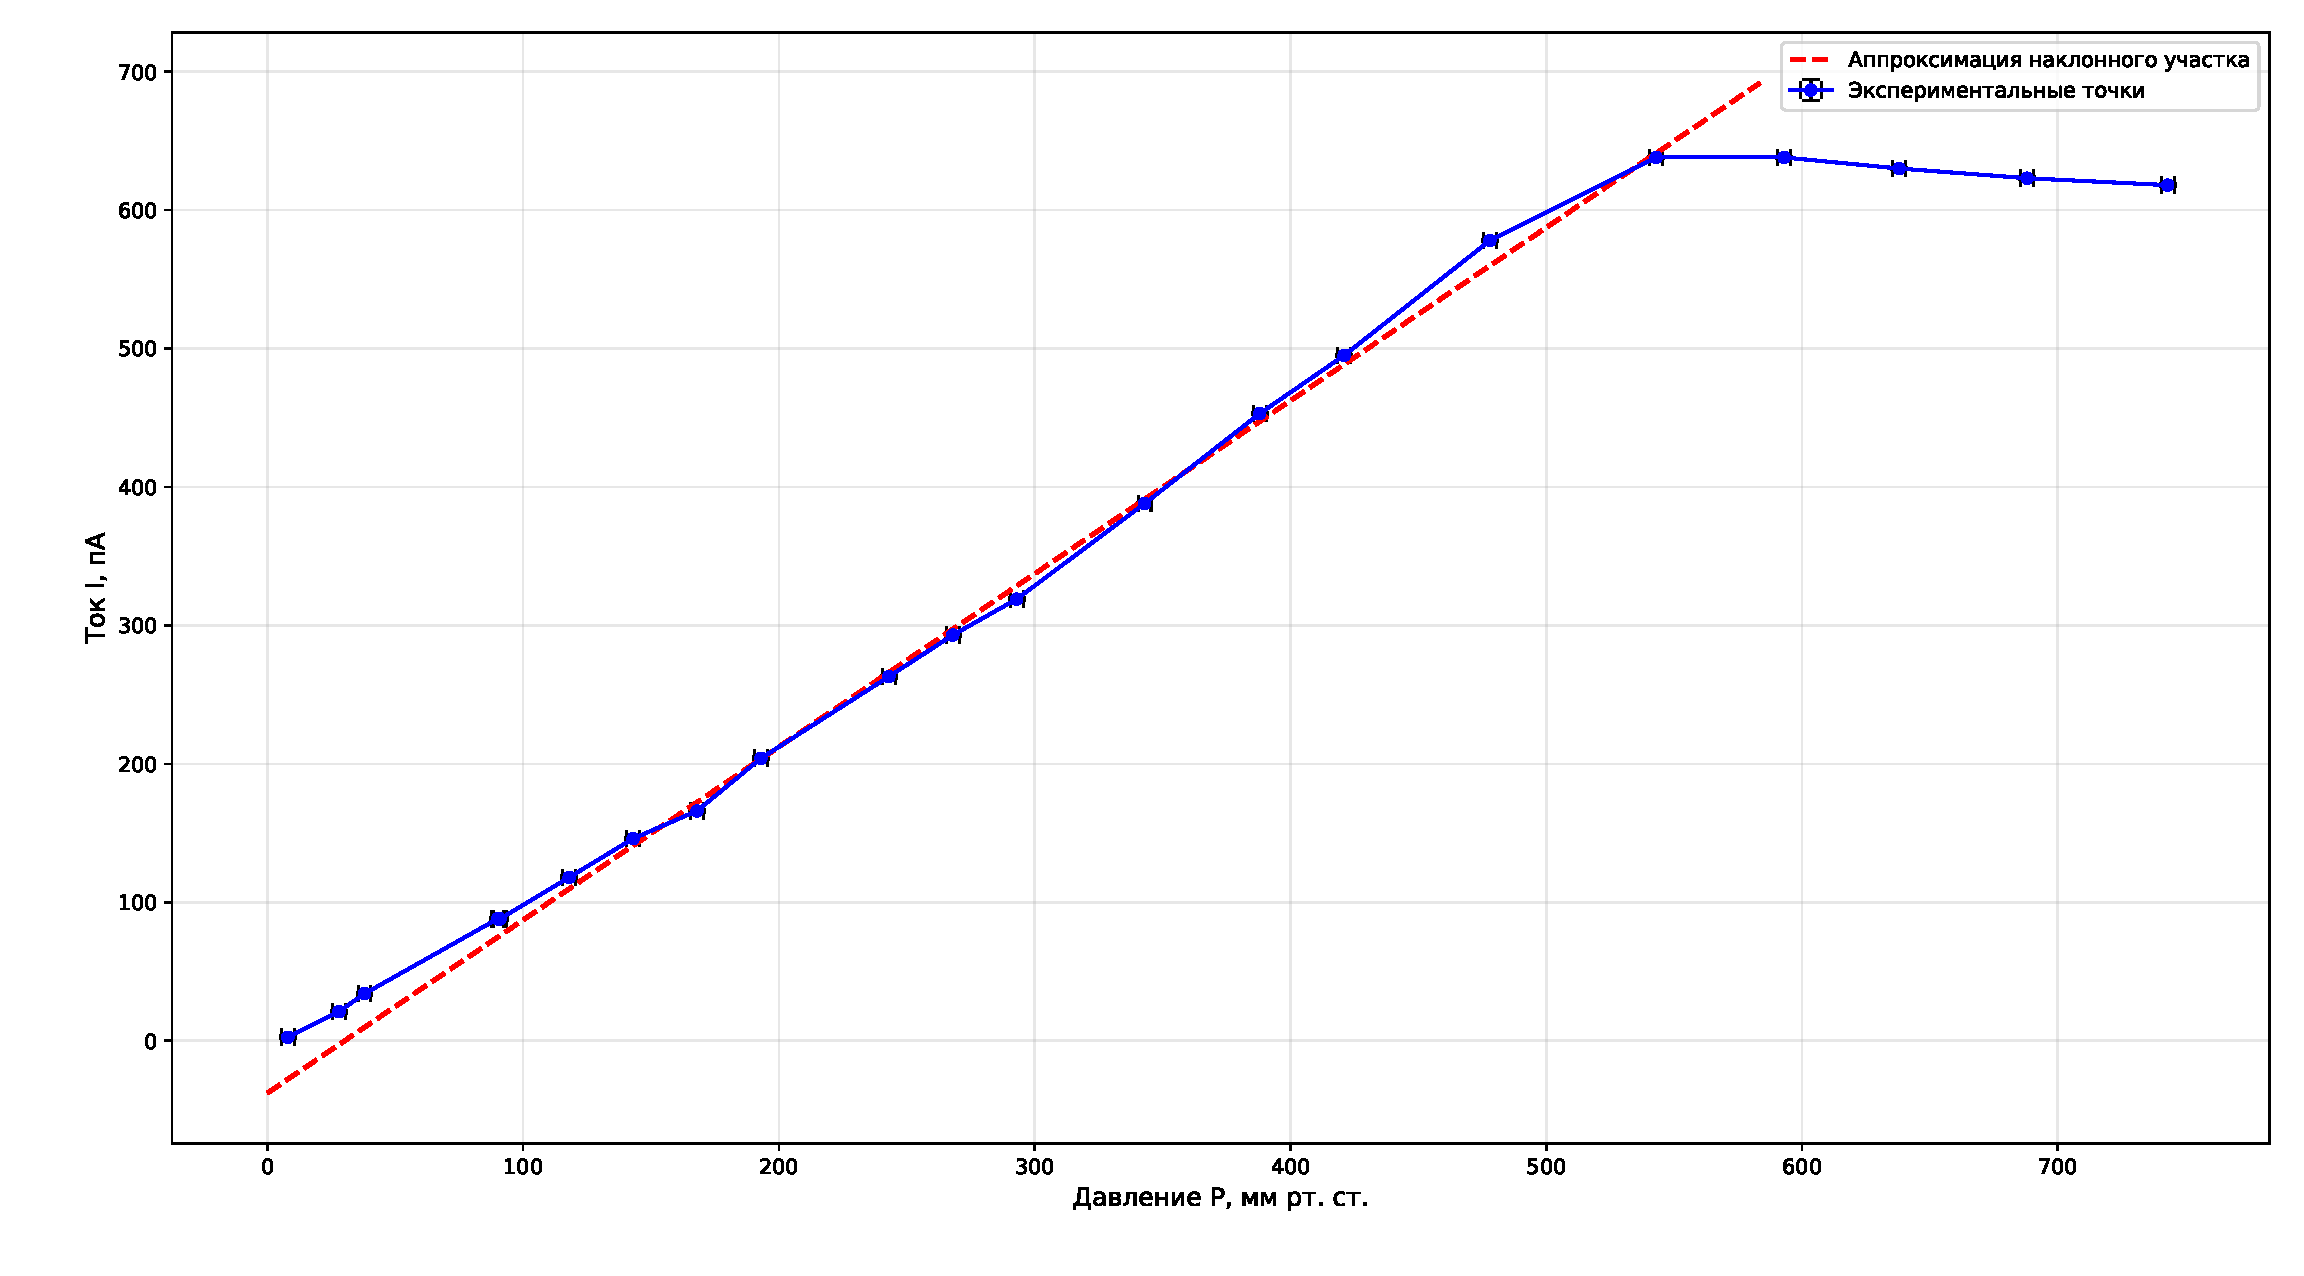
\includegraphics[width=0.8\textwidth]{9.pdf}
    \caption{Зависимость тока ионизационной камеры от давления}
    \label{fig:ion_graph}
\end{figure}

Из графика видно, что при малых давлениях ток растёт примерно линейно, а потом выходит на плато. Чтобы найти экстраполированный пробег, нужно продлить наклонный участок до пересечения с горизонтальным. Из графика получаем:

\begin{equation}
    P_{\text{э}} \approx 520 \text{ мм рт. ст.}
\end{equation}

Теперь пересчитаем пробег к нормальным условиям. Геометрическое расстояние $L$, которое проходят $\alpha$-частицы в камере, определяется конструкцией электродов: внутренний электрод --- диск диаметром 5 мм с нанесенным источником, внешний электрод --- сферическая оболочка с внутренним диаметром 100 мм. $\alpha$-Частицы движутся от диска к стенке шара. Поскольку радиус шара равен 50 мм, а размеры диска малы, принимаем $L \approx 4,75$ см (расстояние от поверхности диска до внутренней стенки сферы).
Формула пересчёта такая же, как во второй части:
\begin{equation}
    R_0 = L \cdot \frac{P_{\text{э}}}{P_0} \cdot \frac{T_0}{T_{\text{оп}}}
\end{equation}

Подставляем: $L = 4,75$ см, $P_{\text{э}} = 520$ мм рт. ст., $P_0 = 760$ мм рт. ст., $T_0 = 288$ К, $T_{\text{оп}} = 293$ К:
\begin{equation}
    R_0 \approx 3,20 \text{ см}
\end{equation}

Массовый пробег:
\begin{equation}
    R'_0 = \rho_0 R_0 \approx 3,92 \cdot 10^{-3} \text{ г/см}^2
\end{equation}

Теперь найдём энергию $\alpha$-частиц по формуле $R = 0,32 E^{3/2}$:
\begin{equation}
    E = \left(\frac{R_0}{0,32}\right)^{2/3} \approx 4,64 \text{ МэВ}
\end{equation}

Табличное значение 5,15 МэВ. Наш результат немного меньше, но это нормально, потому что на источнике есть защитная плёнка, которая забирает часть энергии.

Расхождение: $\frac{5,15 - 4,64}{5,15} \cdot 100\% \approx 10\%$.

Теперь определим, какой толщины бумажный листок не пропустит $\alpha$-частицы. Плотность бумаги примерно 0,8 г/см³. Пробег в бумаге будет таким же по массе, что и в воздухе (3.92 мг/см²). Толщина бумаги:
\begin{equation}
    h = \frac{R'_0}{\rho_{\text{бум}}} \approx 4,9 \cdot 10^{-3} \text{ см} \approx 50 \text{ мкм}
\end{equation}

То есть обычный лист бумаги (толщиной около 0,1 мм) полностью остановит $\alpha$-частицы от плутония.

\subsection*{Вывод}

Результаты экспериментов представлены в таблице:

\begin{table}[H]
\centering
% \caption{Сравнение пробегов, полученных разными методами}
\begin{tabular}{|c|c|c|}
\hline
Метод & $R_0$, см & $E$, МэВ \\
\hline
Счётчик Гейгера & 0,81 & 1,8 \\
Сцинтилляционный счётчик & 2,42 & 3,85 \\
Ионизационная камера & 3,20 & 4,64 \\
Табличное значение & 3,74 & 5,15 \\
\hline
\end{tabular}
\end{table}

Видно, что ионизационная камера дала самый близкий к табличному результат. Это потому что в ней нет слюдяного окошка (как у счётчика Гейгера), и геометрия установки лучше (частицы летят во все стороны внутри камеры, а не через коллиматор).

Сцинтилляционный счётчик тоже дал неплохие результаты, но в нём расстояние фиксированное (9 см), и частицы должны долететь точно до люминофора.

Счётчик Гейгера дал самый маленький пробег из-за слюдяного окошка, которое поглощает часть энергии.

Таким образом, все три метода работают, и ионизационная камера является самой точной для измерения пробега $\alpha$-частиц.













\end{document}